%! TEX program = lualatex
% find: (\\E{$((?!\$}).)+\$)
%replace: \E{\1}

%%%%%%%%%%
% BEAMER %
%%%%%%%%%%

\RequirePackage{luatex85}

\PassOptionsToPackage{luatex}{hyperref}

\documentclass[luatex]{beamer}
%\documentclass[handout]{beamer}

\usetheme{metropolis}

	\newcommand{\bigq}{\mathbb{Q}}
\newcommand{\bb}{\bfseries\large}
\newcommand{\class}{\mathcal}
\newcommand{\mbi}[1]{\textbf{\em{#1}}}
\newcommand{\bi}[1]{\textbf{\textit{#1}}}
\newcommand{\ita}[1]{\textit{#1}}
\newcommand{\p}{\cdot}
\newcommand{\req}{\emptyset}
\newcommand{\init}{\mathcal{J}}
\newcommand{\power}[1]{\class{P}(#1)}
\newcommand{\bigpower}[2]{\class{P}^{#1}(#2)}
\newcommand{\symetric}{\bigtriangleup}
\newcommand{\gx}[3]{\Gamma_{(#1,#2)}(#3)}
\newcommand{\bd}[3]{\Delta_{(#1,#2)}(#3)}
\newcommand{\bp}[3]{\Phi_{(#1,#2)}(#3)}
\newcommand{\eab}{\eta_{\alpha \beta}}
\newcommand{\sab}{\sigma_{\alpha\beta}}
\newcommand{\dab}{\class{D}_{\alpha\beta}}
\newcommand{\cab}{\class{C}_{\alpha\beta}}
\newcommand{\C}[1]{\class{#1}}
\newcommand{\ol}{\overline}
\newcommand{\into}{\longrightarrow}
\newcommand{\ifff}{\Longleftrightarrow}
\newcommand{\imply}{\Rightarrow}
\newcommand{\since}{\Longleftarrow}
\newcommand{\la}{\langle}
\newcommand{\ra}{\rangle}
\newcommand{\andd}{\wedge}
\newcommand{\orr}{\vee}
\newcommand{\ft}{(\C F \C T)_Q}
\newcommand{\pathopen}[3]{#1_{(\ol{#2},#3)}}
\newcommand{\fpi}[3]{#1_*(\Pi(#2,#3))}
\newcommand{\xpath}[2]{(\ol {#1},#2)}
\newcommand{\qn}[2]{\Lambda(#1,#2)}
\newcommand{\jh}{\class J \class H}
\newcommand{\bos}{\boldsymbol}
\newcommand{\f}{\mathbb}
\newcommand{\rss}{\la\psi_i:i\in \lambda\ra}
\newcommand{\ito}[1]{\overset{#1}{\longrightarrow}}
\newcommand{\pcomplex}[2]{\class #1(\class #2)}
\newcommand{\then}{\Rightarrow}
\newcommand{\ud}{{ {up-down-automaton}} }

\newcommand{\map}[1]{\underset{#1}{\mapsto}}
\newcommand{\mapi}[1]{\underset{#1}{\overset{i}{\mapsto}}}
\newcommand{\mapstar}[1]{\underset{#1}{\overset{*}{\mapsto}}}
\newcommand{\mapk}[2]{\underset{#1}{\overset{#2}{\mapsto}}}

\newcommand{\eql}{\equiv_L}
\newcommand{\der}[1]{\underset{#1}{\imply}}
\newcommand{\deri}[1]{\underset{#1}{\overset{i}{\imply}}}
\newcommand{\derstar}[1]{\underset{#1}{\overset{*}{\imply}}}
\newcommand{\derk}[2]{\underset{#1}{\overset{#2}{\imply}}}
\newcommand{\blank}{\bar{b}}
\newcommand{\R}[1]{#1}
\newcommand{\say}[1]{\color{blue}{#1}\color{black}}



% Fix the title separator
\makeatletter
\setbeamertemplate{title separator}{
	\bgroup
	\bodydir TLT
	\begin{tikzpicture}
	\fill[fg] (0,0) rectangle (\textwidth, \metropolis@titleseparator@linewidth);
	\end{tikzpicture}%
	\egroup
	\par%
}
\makeatother

% Fix the progress bar and make it progress from right to left
\makeatletter
\setbeamertemplate{progress bar in section page}{
	\setlength{\metropolis@progressonsectionpage}{%
		\textwidth * \ratio{\insertframenumber pt}{\inserttotalframenumber pt}%
	}%
	\bgroup
	\bodydir TLT
	\begin{tikzpicture}
	\fill[bg] (0,0) rectangle (\textwidth, \metropolis@progressonsectionpage@linewidth);
	\fill[fg] (\textwidth,0) rectangle (\textwidth-\metropolis@progressonsectionpage, \metropolis@progressonsectionpage@linewidth);
	\end{tikzpicture}%
	\egroup
}
\makeatother

% A more logical title page, juxtaposing `institute` to `author`. This modification is not necessary for Hebrew support.
\makeatletter
\setbeamertemplate{title page}{
	\begin{minipage}[b][\paperheight]{\textwidth}
		\ifx\inserttitlegraphic\@empty\else\usebeamertemplate*{title graphic}\fi
		\vfill%
		\ifx\inserttitle\@empty\else\usebeamertemplate*{title}\fi
		\ifx\insertsubtitle\@empty\else\usebeamertemplate*{subtitle}\fi
		\usebeamertemplate*{title separator}
		\ifx\beamer@shortauthor\@empty\else\usebeamertemplate*{author}\fi
		\ifx\insertinstitute\@empty\else\usebeamertemplate*{institute}\fi
		\ifx\insertdate\@empty\else\usebeamertemplate*{date}\fi
		\vfill
		\vspace*{1mm}
	\end{minipage}
}
\setbeamertemplate{author}{\vspace*{2em}\insertauthor\par\vspace*{0.25em}}
\setbeamertemplate{institute}{\insertinstitute\par}
\setbeamertemplate{date}{\vspace*{3mm}\insertdate\par}
\makeatother




%%%%%%%%%
% Babel %
%%%%%%%%%

\usepackage[nil,bidi=basic-r]{babel}
\babelprovide[import=he,main]{hebrew}
\babelprovide[import=en-GB]{english}

% For some reason Babel’s `\babelfont` doesn’t work
\setsansfont[Script=Hebrew]{Open Sans Hebrew}
\setmonofont{Fira Mono}
\renewcommand{\H}[1]{\foreignlanguage{hebrew}{\fontspec[Script=Hebrew]{Open Sans Hebrew}#1}}
\newcommand{\E}[1]{\foreignlanguage{english}{\fontspec{Open Sans}#1}}
\newcommand{\LR}[1]{{‏\textdir TLT #1}}




%%%%%%%%
% MISC %
%%%%%%%%

\usepackage{metalogo, fancyvrb}
\usepackage{cancel}
\newcommand{\smallurl}[1]{{\footnotesize\url{#1}}}



%%%%%%%%%%%%
% DOCUMENT %
%%%%%%%%%%%%

\begin{document}
	\title{מבוא והגדרות}
	\subtitle{מפגש 1}
	%\author{}
	%\institute{}
	\date{}
	
 \section{ברוכים הבאים לקורס אלגוריתמים!}
%אני אורן
% הרצאתי בעבר בבן גוריון שם סיימתי את התואר השני שלי וכעת זו הפעם הראשונה שאני מלמד באו"פ
%כיוונתי ובחרתי ללמד את הקורס הזה כי זה אחד מהקורסים שאני אישית שהכי נהנתי בו בתואר
%אני אוהב ללמד ולכן אני משקיע המון בצורה שבה החומר יועבר
%אתם תמיד מוזמנים לבוא לשאול שאלות ולתת לי פידבק על ההרצאות
%אם זה לא באונברסיטה בטח תוכלו לפגוש אותי ב...
%ואם אני לא עונה לכם מיד כנראה ש זה בגלל שאני עם הבן שלי נאל בן שנה וחצי 	

\begin{frame}
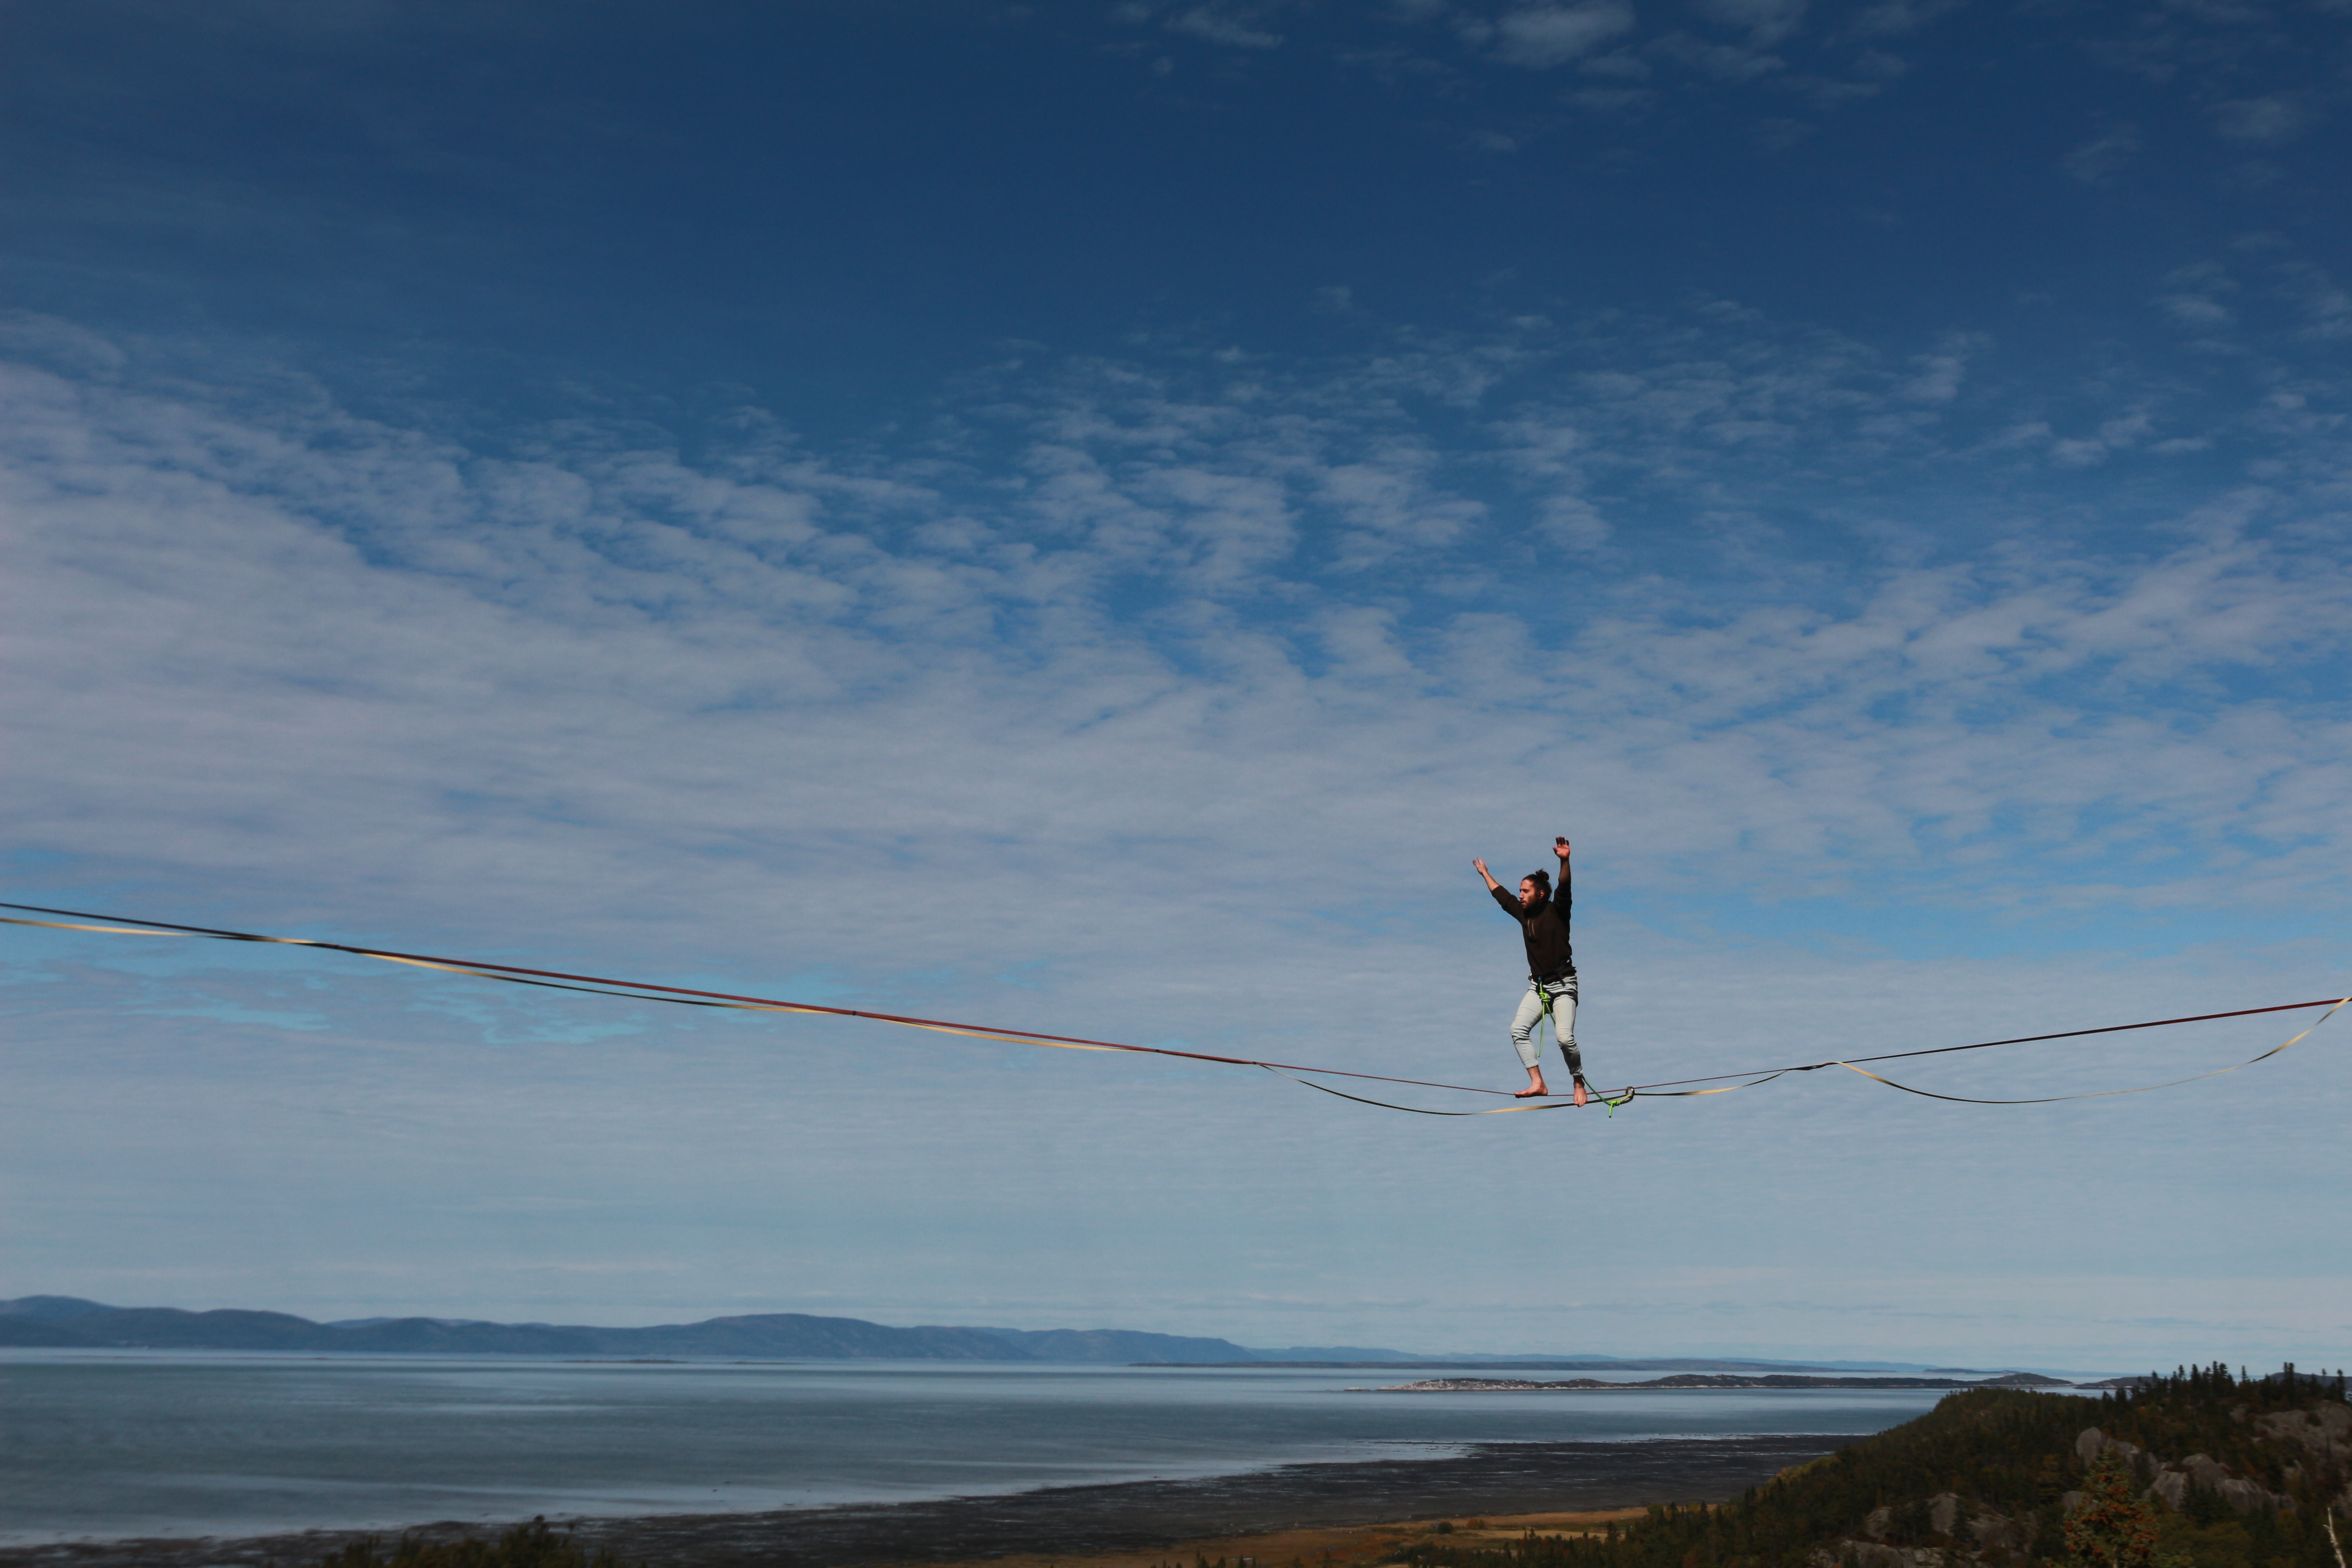
\includegraphics[width=\linewidth]{imgs/highline.jpg}
\end{frame}
\begin{frame}
\includegraphics[width=\linewidth]{imgs/nael.jpg}
\end{frame}
\section{מה אתם עושים פה? \\ \large{(או - מה אתם חושבים שנעשה פה)}}
%\url{https://www.menti.com/9cgyhmrxt9}
% הצגה של התלמידים
\section{ברוכים הבאים לקורס  טעימות של אלגוריתמים!}
\section{מהי התרומה של הקורס עבורכם?}
% ממקצע אותנו בלהוכיח הוכחות פורמליות
% 
% עוזר לסיים את התואר
% מפגיש אותנו עם אלגורתמים שימושיים לתעשייה
 \section{אנשים אומרים שאלגוריתמים הוא אחד הקורס 
 \textit{הקשים בתואר}
}
  \section{הם צודקים.}
  \begin{frame}
  \begin{figure}
  	\centering
  	\includegraphics[width=1\linewidth]{imgs/hard}
  	\label{fig:hard}
  \end{figure}
  \end{frame}
\begin{frame}{דברים שנגיד פעם אחת}
\pause
\begin{itemize}[<+->]
	\item \url{oren.roth@openu.ac.il}
	\item שעת הנחייה: שלישי 14:00-15:00, 0542244598
	\item אתר הקורס
	\item   ממ"ן ומבחן
	\begin{itemize}[<+->]
		\item כל המידע הטכני מופיע בחוברת הקורס
		\item לכל ממ"ן יהיה פורום באתר בו תוכלו לשאול שאלות
	\end{itemize}
\end{itemize}
\end{frame}
\begin{frame}{איך נגרום לזה לעבוד?}
\pause
\begin{itemize}[<+->]
\item לפני כל שיעור תקראו את החומר (לפי לוח הזמנים שמופיע בחוברת הקורס)
	\begin{itemize}[<+->]
	\item  אנחנו נדבר בקצרה על חומרים מתוך פרקים  1-2
	\item ב2-3 שבועות הראשונים נתחיל בפרק 3
\end{itemize}
\item תשלחו שאלות ונושאים שדורשים הבהרות למייל שלי לפני השיעור
\item "מי שמבין חומר בצורה עמוקה יכול להסביר אותו בצורה פשוטה"
	\note{
		 אם משהו לא מובן (בפרט ייתכן שאני אומר מושג שעבורי זה טרוואילי)
		 הפנו את תשומת ליבי ואני אגיד אותו בעברית פשוטה.
}
\item מה עוזר לכם ללמוד חומר מורכב?
\end{itemize}
\end{frame}
\begin{frame}{התוכנית שלנו להיום}
\pause
\begin{itemize}[<+->]
	\item מבוא והגדרות בסיסיות 
	\item חזרה מהירה על ניתוח זמני ריצה
	\item מושגים בסיסיים מעולם הגרפים
\end{itemize}
\end{frame}
\section{\#התחלנו}
\part{מבוא והגדרות בסיסיות}
\frame{\partpage}
\begin{frame}{בעיה, מופע ופתרון}
\begin{figure}
	\centering
	\includegraphics[width=0.7\linewidth]{imgs/screenshot001.jpg}
\end{figure}

\end{frame}
 \section{מה זה אלגוריתם?}
\begin{frame}{מה זה אלגוריתם?}



\pause
\begin{itemize}[<+->]
	\item סדרה של פעולות
	\item בסיומה מוחזר פלט
	\item בקורס אנחנו מתרכזים רק באלגורתמים שתמיד מחזירים תשובה נכונה \textbf{לכל מופע}
\end{itemize}
\end{frame}
 \section{הוכחת נכונות פורמאלית}
 	\note{1. מאוד פורמלי ומרגיש לא טבעי אבל לאט לאט זה יתברר כמאוד שימושי לשיח בנינו ויראה דווקא מאוד שימוש
 	
 	2. טענה ראשית - ט"ע וכ"ו - למה זה טוב}

\begin{frame}{דוגמא}
 נתון אלגוריתם אשר "לכל מפת כבישים, עיר מוצא ועיר יעד, האלגוריתם יחזיר מסלול קצר ביותר במפה בין שתי הערים". 
\pause עלינו להוכיח כי האלגוריתם אכן מקיים את הטענה לעיל תחת שני מקרים:
\pause
\begin{itemize}[<+->]
	\item 	ישנו מסלול במפת הכבישים בין שתי ערים נתונות.
\item 	במפת הכבישים אין מסלול בין שתי ערים נתונות.
\end{itemize}

\end{frame}
 \begin{frame}{זמני ריצה}
 \pause
 להלן כמה דוגמאות לזמני ריצה, כאשר $n$ מסמל את גודל המופע:
  \pause
 \begin{itemize}[<+->]
 	\item 	 \E{$O(1)$} - זמן ריצה קבוע.  \pause בעיות שניתנות לפיתרון בזמן קבוע (כלומר אינו תלוי בגודל הקלט). לרוב, אינן מעניינות במיוחד.  \pause
\item \E{$O(log~n)$}   - זמן לוגריתמי.
\item \E{$O(n)$}   - זמן לינארי.
\item \E{$O(n^c)$}   - עבור \E{$c\in \mathbb N$} - זמן פולינומי.
\item \E{$O(2^{cn})$}   - עבור \E{$c\in \mathbb N$} - זמן אקספוננציאלי.   \pause זמן זה נחשב ללא יעיל במיוחד, כאשר הזמן הדרוש לפתרון של קלטים קטנים יחסית יכול להיות עצום.
\pause
\item *הביטו בטבלה 2.1 בספר (עמוד 39)
 \end{itemize}
\end{frame}
\begin{frame}{כתיבת אלגוריתם בשלושה חלקים}
בבואנו לכתוב אלגוריתם הפותר בעיה נתייחס לשלושה אספקטים:
 \pause
\begin{enumerate}[<+->]
	\item תיאור דרך כללית להגעה לפתרון עבור מופע כלשהו של הבעיה (ע"י תיאור אלגוריתם).
	\item הוכחת נכונות הדרך שתיארנו (על ידי הוכחה {פורמאלית}).
	\item ניתוח זמן הריצה הדרוש לקבלת הפתרון, בהתאם לדרך שתיארנו.
\end{enumerate}

\end{frame}

\part{מושגים בסיסיים מעולם הגרפים}
\frame{\partpage}
\begin{frame}{מושגים בסיסיים}
\pause
\begin{itemize}[<+->]
	\item  גרף לא מכוון הוא זוג
	\E{$G=(V,E)$}
	\begin{itemize}[<+->]


	\item $V$ היא קבוצה סופית של איברים הנקראים צמתים
או קודקודים.

	\item \E{$E$} היא קבוצה של זוגות לא סדורים מתוך \E{$V$} 
	הנקראים קשתות.
	\end{itemize}

\end{itemize}
\begin{figure}
	\centering
	\includegraphics[width=0.7\linewidth]{imgs/graph}
	\label{fig:graph}
\end{figure}

\end{frame}

\begin{frame}{מושגים בסיסיים}
\pause
\begin{itemize}[<+->]
	\item \textbf{שכן - } צומת \E{$v$} הוא שכן של צומת \E{$u$}, אם קיימת קשת בגרף \E{$\{u,v\}$}, היחס כמובן סימטרי.
	\item  \textbf{דרגה - } הדרגה של צומת \E{$u$} שווה למספר השכנים של \E{$u$} ומסומנת  \E{$deg(u)$}.
	
		\item  \textbf{מסלול - } מסלול בגרף הוא סדרה של צמתים 
		\E{$(v_1,\ldots,v_k)$}
		שבה כל זוג 
		\E{$(v_i,v_{i+1})$}
		היא קשת בגרף.
	
\end{itemize}
\end{frame}
\begin{frame}{מושגים בסיסיים}
\pause
\begin{itemize}[<+->]
\item \textbf{אורך מסלול - } מספר הקשתות במסלול. אורך המסלול 
\E{$(v_1,\ldots,v_k)$}
הוא
\E{$k-1$}
\item  \textbf{מרחק בין צמתים - } אורך המסלול הקצר
ביותר המחבר אותם. אם אין מסלול כזה,  המרחק מוגדר להיות אינסוף.

\item  \textbf{מסלול פשוט- } 
 מסלול בו שום צומת איננו
מופיע יותר מפעם אחת. 

\end{itemize}

\end{frame}

\begin{frame}{מושגים בסיסיים}
\pause
\begin{itemize}[<+->]
	\item \textbf{מעגל - } מסלול המכיל לפחות שלושה צמתים
שונים ובו הצומת הראשון והאחרון זהים, כל  שאר הצמתים במסלול מופיעים בדיוק פעם אחת.
	\item  \textbf{גרף קשיר - }
	גרף נקרא קשיר אם בין כל זוג
צמתים בגרף קיים מסלול המקשר אותם. 
	\item  \textbf{תת-גרף- } 
\E{$H=(V',E')$}
	נקרא תת-גרף של הגרף
	\E{$G=(V,E)$}
, אם
\E{$H$}
הוא גרף וגם,
\E{$E'\subseteq E,\quad V'\subseteq V$}

	
\end{itemize}

\end{frame}


\begin{frame}{מושגים בסיסיים}
\pause
\begin{itemize}[<+->]
	\item \textbf{עץ –} 
	גרף קשיר ללא מעגלים.
	\item \textbf{עץ מושרש –}
	 עץ עם שורש מיוחד הנקרא
 שורש. צומת
 \E{$v$} 
  הוא צאצא של צומת
   \E{$u$}
    אם
       \E{$u$}
     מופיע על המסלול הפשוט (היחיד) המחבר את
      \E{$v$} 
       לשורש.
	
\end{itemize}

\end{frame}

\begin{frame}{מושגים בסיסיים - גרפים מכוונים}
\pause
\begin{itemize}[<+->]
	\item  \textbf{גרף מכוון} הוא זוג
	\E{$G=(V,E)$}
	\begin{itemize}[<+->]
		
		
		\item $V$ היא קבוצה סופית של איברים הנקראים צמתים
		או קודקודים.
		
		\item \E{$E$} היא קבוצה של זוגות \textbf{סדורים} מתוך \E{$V$} 
		הנקראים קשתות.
	\end{itemize}
	
\end{itemize}
\begin{figure}
	\centering
	\includegraphics[width=0.7\linewidth]{imgs/directed-graph}
	\label{fig:directed-graph}
\end{figure}


\end{frame}

\begin{frame}{מושגים בסיסיים - גרפים מכוונים}
\pause
\begin{itemize}[<+->]
	\item  \textbf{דרגת כניסה של צומת 
		\E{$v$}
		 – } 
	מספר הקשתות
הנכנסות ל
		\E{$v$}
.
\item  \textbf{דרגת יציאה של צומת 
	\E{$v$}
	– } 
מספר הקשתות
היוצאות מ
\E{$v$}
.
	\item  \textbf{DAG}  גרף מכוון ללא
מעגלים מכוונים בגרף.

		\item  \textbf{קשירות היטב - }
				\E{$u$}
		ו-
				\E{$v$}
		קשירים היטב, אם קיים מסלול מכוון מ
				\E{$u$}
		ל
				\E{$v$}
		וכמו כן מ
				\E{$v$}
		ל
				\E{$u$}
		. 

	
\end{itemize}


\end{frame}
\begin{frame}{שאלה 1}
\pause
\begin{itemize}[<+->]
	\item נקרא למסלול "מסלול פשוט קשתות" אמ"מ אין בו
קשת החוזרת פעמיים

	\item הוכח או הפרך ע"י מתן דוגמא נגדית
\begin{itemize}[<+->]
	\item האם כל מסלול פשוט הוא מסלול פשוט קשתות?
	\begin{itemize}[<+->]
		\item נכון. נניח בשלילה שלא.
אזי במסלול קיימת קשת המופיעה פעמיים במסלול, ולכן הקודקדים  הסמוכים לה מופעים פעמים, והמסלול אינו פשוט, בסתירה להנחה.
	\end{itemize}
\item האם כל מסלול פשוט-קשתות הוא מסלול פשוט?
\begin{itemize}[<+->]
	\item לא נכון. להלן דוגמא נגדית
\end{itemize}	
\pause
\begin{figure}
	\centering
	\includegraphics[width=0.2\linewidth]{imgs/counter-example}
	\label{fig:counter-example}
\end{figure}

\end{itemize}
\end{itemize}
\end{frame}
\begin{frame}{גרפים}
\pause
\begin{itemize}[<+->]
	\item מבני נתונים לשמירת גרפים:
\begin{itemize}[<+->]
	\item מטריצת סמיכויות
	\item רשימת סמיכויות
\end{itemize}
\end{itemize}	
\end{frame}
\begin{frame}{מטריצת סמיכויות - דוגמא}
\pause
\begin{center}
	\includegraphics[width=0.4\linewidth]{imgs/matrix1}
\end{center}
\begin{center}
	\includegraphics[width=0.4\linewidth]{imgs/matrix2}
\end{center}
\end{frame}
\begin{frame}{מטריצת סמיכויות:}
\begin{itemize}[<+->]
	\item מטריצה
	\E{$A=(a_{ij})$}
	שמימדיה
	\E{$|V|\times |V|$}
	וערכי איבריה:
	\begin{figure}
		\centering
		\includegraphics[width=0.5\linewidth]{imgs/case}
		\label{fig:case}
	\end{figure}
	
	\item הייצוג ע"י מטריצת סמיכויות עשוי להיות עדיף כאשר
הגרף צפוף או כאשר נדרשת היכולת לגלות במהירות אם  קיימת קשת המחברת שני קודקודים נתונים.
\end{itemize}
\end{frame}

\begin{frame}{רשימת סמיכויות - דוגמא}
\begin{center}
	\includegraphics[width=0.4\linewidth]{imgs/matrix1}
\end{center}
\begin{center}
	\includegraphics[width=0.4\linewidth]{imgs/list}
\end{center}
\end{frame}
\begin{frame}{רשימת סמיכויות}
\pause
\begin{itemize}[<+->]
	\item הייצוג ע"י רשימות סמיכות של גרף
	\E{$G = (V, E)$}
	מורכב
	ממערך
	\E{Adj}
	של
	\E{$|V|$}
	רשימות, אחת עבור כל קדקוד ב-
	\E{$V$}.
	\item  עבור כל
	\E{$u$}
	מ-
	\E{$V$}
	רשימת
	\E{$Adj[u]$}
	מכילה מצביעים לכל הקודקודים
	\E{$v$}
	שעבורם קיימת קשת
\E{$(u,v)$}
	.
	\item   בד"כ קודקודים
	בכל רשימת סמיכות מאוחסנים בסדר שרירותי.
\end{itemize}

  \end{frame}

\begin{frame}{עלות מקום לייצוגים}
\pause
\begin{itemize}[<+->]
	\item 
	עלות המקום כאשר מייצגים גרף בעזרת
 
מטריצת סמיכויות: 
\E{$\Theta(|V|^2)$}
	\item  ובייצוג על ידי רשימת סמיכויות:
	\E{$\Theta(|V|+|E|)$}
\end{itemize}
\end{frame}
\begin{frame}
\vspace*{-1pt}
\makebox[\linewidth]{\includegraphics[page=25,width=\paperwidth]{pdfs/lec1}}
\end{frame}

\begin{frame}
\vspace*{-1pt}
\makebox[\linewidth]{\includegraphics[page=26,width=\paperwidth]{pdfs/lec1}}
\end{frame}
\begin{frame}{טכניקות בסיסיות ושימושיות מאוד}
\pause
\begin{itemize}[<+->]
	\item אינדוקציה
	\item עקרון שובך היונים: אם מכניסים
	\E{$n+1$}
	ל
	\E{$n$}
שובכים אז קיים שובך אחד בו לפחות 2 יונים.\\\pause
שימוש: כל מסלול בגרף בעלת
\E{$n+1$}
קודקודים מכילה מעגל.\pause
	\item בגרף לא מכוון:
$$\sum_{v\in V} deg(v) = 2|E|$$
\end{itemize}
\end{frame}
\begin{frame}{שאלה 2}
הראה שבכל גרף בלתי מכוון וקשיר 
\E{$|E|\ge |V|-1$}
\end{frame}
%\begin{frame}
%\vspace*{-1pt}
%\makebox[\linewidth]{\includegraphics[page=29,width=\paperwidth]{pdfs/lec1}}
%\end{frame}
\begin{frame}{שאלה 3}
הראו שבכל DAG (גרף מכוון חסר מעגלים) יש קודקוד מקור (קודקוד שדרגת הכניסה אליו היא 0)
\end{frame}
%BFS STARTS
\begin{frame}
\vspace*{-1pt}
\makebox[\linewidth]{\includegraphics[page=34,width=\paperwidth]{pdfs/lec1}}
\end{frame}
\begin{frame}
\vspace*{-1pt}
\makebox[\linewidth]{\includegraphics[page=35,width=\paperwidth]{pdfs/lec1}}
\end{frame}
\begin{frame}
\vspace*{-1pt}
\makebox[\linewidth]{\includegraphics[page=36,width=\paperwidth]{pdfs/lec1}}
\end{frame}
\begin{frame}
\vspace*{-1pt}
\makebox[\linewidth]{\includegraphics[page=37,width=\paperwidth]{pdfs/lec1}}
\end{frame}
\begin{frame}
\vspace*{-1pt}
\makebox[\linewidth]{\includegraphics[page=38,width=\paperwidth]{pdfs/lec1}}
\end{frame}
\begin{frame}
\vspace*{-1pt}
\makebox[\linewidth]{\includegraphics[page=39,width=\paperwidth]{pdfs/lec1}}
\end{frame}
\begin{frame}
\vspace*{-1pt}
\makebox[\linewidth]{\includegraphics[page=40,width=\paperwidth]{pdfs/lec1}}
\end{frame}
\begin{frame}
\vspace*{-1pt}
\makebox[\linewidth]{\includegraphics[page=41,width=\paperwidth]{pdfs/lec1}}
\end{frame}
\begin{frame}
\vspace*{-1pt}
\makebox[\linewidth]{\includegraphics[page=42,width=\paperwidth]{pdfs/lec1}}
\end{frame}
\begin{frame}
\vspace*{-1pt}
\makebox[\linewidth]{\includegraphics[page=43,width=\paperwidth]{pdfs/lec1}}
\end{frame}
\begin{frame}
\vspace*{-1pt}
\makebox[\linewidth]{\includegraphics[page=44,width=\paperwidth]{pdfs/lec1}}
\end{frame}
\begin{frame}
\vspace*{-1pt}
\makebox[\linewidth]{\includegraphics[page=45,width=\paperwidth]{pdfs/lec1}}
\end{frame}
\begin{frame}
\vspace*{-1pt}
\makebox[\linewidth]{\includegraphics[page=46,width=\paperwidth]{pdfs/lec1}}
\end{frame}
\begin{frame}
\vspace*{-1pt}
\makebox[\linewidth]{\includegraphics[page=47,width=\paperwidth]{pdfs/lec1}}
\end{frame}
\begin{frame}
\vspace*{-1pt}
\makebox[\linewidth]{\includegraphics[page=48,width=\paperwidth]{pdfs/lec1}}
\end{frame}
\begin{frame}
\vspace*{-1pt}
\makebox[\linewidth]{\includegraphics[page=49,width=\paperwidth]{pdfs/lec1}}
\end{frame}
\begin{frame}
\vspace*{-1pt}
\makebox[\linewidth]{\includegraphics[page=50,width=\paperwidth]{pdfs/lec1}}
\end{frame}
\begin{frame}
\vspace*{-1pt}
\makebox[\linewidth]{\includegraphics[page=51,width=\paperwidth]{pdfs/lec1}}
\end{frame}
\begin{frame}
\vspace*{-1pt}
\makebox[\linewidth]{\includegraphics[page=52,width=\paperwidth]{pdfs/lec1}}
\end{frame}
\begin{frame}
\vspace*{-1pt}
\makebox[\linewidth]{\includegraphics[page=53,width=\paperwidth]{pdfs/lec1}}
\end{frame}
\begin{frame}
\vspace*{-1pt}
\makebox[\linewidth]{\includegraphics[page=54,width=\paperwidth]{pdfs/lec1}}
\end{frame}
\begin{frame}
\vspace*{-1pt}
\makebox[\linewidth]{\includegraphics[page=55,width=\paperwidth]{pdfs/lec1}}
\end{frame}
\begin{frame}
\vspace*{-1pt}
\makebox[\linewidth]{\includegraphics[page=56,width=\paperwidth]{pdfs/lec1}}
\end{frame}
\begin{frame}
\vspace*{-1pt}
\makebox[\linewidth]{\includegraphics[page=57,width=\paperwidth]{pdfs/lec1}}
\end{frame}
\begin{frame}
\vspace*{-1pt}
\makebox[\linewidth]{\includegraphics[page=58,width=\paperwidth]{pdfs/lec1}}
\end{frame}
\begin{frame}
\vspace*{-1pt}
\makebox[\linewidth]{\includegraphics[page=59,width=\paperwidth]{pdfs/lec1}}
\end{frame}
\begin{frame}
\vspace*{-1pt}
\makebox[\linewidth]{\includegraphics[page=60,width=\paperwidth]{pdfs/lec1}}
\end{frame}
\begin{frame}
\vspace*{-1pt}
\makebox[\linewidth]{\includegraphics[page=61,width=\paperwidth]{pdfs/lec1}}
\end{frame}
\begin{frame}
\vspace*{-1pt}
\makebox[\linewidth]{\includegraphics[page=62,width=\paperwidth]{pdfs/lec1}}
\end{frame}
\begin{frame}
\vspace*{-1pt}
\makebox[\linewidth]{\includegraphics[page=63,width=\paperwidth]{pdfs/lec1}}
\end{frame}
\begin{frame}
\vspace*{-1pt}
\makebox[\linewidth]{\includegraphics[page=64,width=\paperwidth]{pdfs/lec1}}
\end{frame}
\begin{frame}
\vspace*{-1pt}
\makebox[\linewidth]{\includegraphics[page=65,width=\paperwidth]{pdfs/lec1}}
\end{frame}
\begin{frame}
\vspace*{-1pt}
\makebox[\linewidth]{\includegraphics[page=66,width=\paperwidth]{pdfs/lec1}}
\end{frame}
\begin{frame}
\vspace*{-1pt}
\makebox[\linewidth]{\includegraphics[page=67,width=\paperwidth]{pdfs/lec1}}
\end{frame}
\begin{frame}
\vspace*{-1pt}
\makebox[\linewidth]{\includegraphics[page=68,width=\paperwidth]{pdfs/lec1}}
\end{frame}
\begin{frame}
\vspace*{-1pt}
\makebox[\linewidth]{\includegraphics[page=69,width=\paperwidth]{pdfs/lec1}}
\end{frame}
\begin{frame}
\vspace*{-1pt}
\makebox[\linewidth]{\includegraphics[page=70,width=\paperwidth]{pdfs/lec1}}
\end{frame}
\begin{frame}
\vspace*{-1pt}
\makebox[\linewidth]{\includegraphics[page=71,width=\paperwidth]{pdfs/lec1}}
\end{frame}
\begin{frame}
\vspace*{-1pt}
\makebox[\linewidth]{\includegraphics[page=72,width=\paperwidth]{pdfs/lec1}}
\end{frame}
\begin{frame}
\vspace*{-1pt}
\makebox[\linewidth]{\includegraphics[page=73,width=\paperwidth]{pdfs/lec1}}
\end{frame}
\begin{frame}
\vspace*{-1pt}
\makebox[\linewidth]{\includegraphics[page=74,width=\paperwidth]{pdfs/lec1}}
\end{frame}
\begin{frame}
\vspace*{-1pt}
\makebox[\linewidth]{\includegraphics[page=75,width=\paperwidth]{pdfs/lec1}}
\end{frame}
\begin{frame}
\vspace*{-1pt}
\makebox[\linewidth]{\includegraphics[page=76,width=\paperwidth]{pdfs/lec1}}
\end{frame}
\begin{frame}
\vspace*{-1pt}
\makebox[\linewidth]{\includegraphics[page=77,width=\paperwidth]{pdfs/lec1}}
\end{frame}
\begin{frame}
\vspace*{-1pt}
\makebox[\linewidth]{\includegraphics[page=78,width=\paperwidth]{pdfs/lec1}}
\end{frame}
\begin{frame}
\vspace*{-1pt}
\makebox[\linewidth]{\includegraphics[page=79,width=\paperwidth]{pdfs/lec1}}
\end{frame}
\begin{frame}
\vspace*{-1pt}
\makebox[\linewidth]{\includegraphics[page=80,width=\paperwidth]{pdfs/lec1}}
\end{frame}
\begin{frame}
\vspace*{-1pt}
\makebox[\linewidth]{\includegraphics[page=81,width=\paperwidth]{pdfs/lec1}}
\end{frame}
\begin{frame}
\vspace*{-1pt}
\makebox[\linewidth]{\includegraphics[page=82,width=\paperwidth]{pdfs/lec1}}
\end{frame}
\begin{frame}
\vspace*{-1pt}
\makebox[\linewidth]{\includegraphics[page=83,width=\paperwidth]{pdfs/lec1}}
\end{frame}
\begin{frame}
\vspace*{-1pt}
\makebox[\linewidth]{\includegraphics[page=84,width=\paperwidth]{pdfs/lec1}}
\end{frame}
\begin{frame}
\vspace*{-1pt}
\makebox[\linewidth]{\includegraphics[page=85,width=\paperwidth]{pdfs/lec1}}
\end{frame}
\begin{frame}
\vspace*{-1pt}
\makebox[\linewidth]{\includegraphics[page=86,width=\paperwidth]{pdfs/lec1}}
\end{frame}
\begin{frame}
\vspace*{-1pt}
\makebox[\linewidth]{\includegraphics[page=87,width=\paperwidth]{pdfs/lec1}}
\end{frame}
\begin{frame}
\vspace*{-1pt}
\makebox[\linewidth]{\includegraphics[page=88,width=\paperwidth]{pdfs/lec1}}
\end{frame}
\begin{frame}
\vspace*{-1pt}
\makebox[\linewidth]{\includegraphics[page=89,width=\paperwidth]{pdfs/lec1}}
\end{frame}
\begin{frame}
\vspace*{-1pt}
\makebox[\linewidth]{\includegraphics[page=90,width=\paperwidth]{pdfs/lec1}}
\end{frame}
\begin{frame}
\vspace*{-1pt}
\makebox[\linewidth]{\includegraphics[page=91,width=\paperwidth]{pdfs/lec1}}
\end{frame}
\begin{frame}
\vspace*{-1pt}
\makebox[\linewidth]{\includegraphics[page=92,width=\paperwidth]{pdfs/lec1}}
\end{frame}
\begin{frame}
\vspace*{-1pt}
\makebox[\linewidth]{\includegraphics[page=93,width=\paperwidth]{pdfs/lec1}}
\end{frame}
\begin{frame}
\vspace*{-1pt}
\makebox[\linewidth]{\includegraphics[page=94,width=\paperwidth]{pdfs/lec1}}
\end{frame}
\begin{frame}
\vspace*{-1pt}
\makebox[\linewidth]{\includegraphics[page=95,width=\paperwidth]{pdfs/lec1}}
\end{frame}
\begin{frame}
\vspace*{-1pt}
\makebox[\linewidth]{\includegraphics[page=96,width=\paperwidth]{pdfs/lec1}}
\end{frame}
\begin{frame}
\vspace*{-1pt}
\makebox[\linewidth]{\includegraphics[page=97,width=\paperwidth]{pdfs/lec1}}
\end{frame}
\begin{frame}
\vspace*{-1pt}
\makebox[\linewidth]{\includegraphics[page=98,width=\paperwidth]{pdfs/lec1}}
\end{frame}
\begin{frame}
\vspace*{-1pt}
\makebox[\linewidth]{\includegraphics[page=99,width=\paperwidth]{pdfs/lec1}}
\end{frame}
\begin{frame}
\vspace*{-1pt}
\makebox[\linewidth]{\includegraphics[page=100,width=\paperwidth]{pdfs/lec1}}
\end{frame}
\begin{frame}
\vspace*{-1pt}
\makebox[\linewidth]{\includegraphics[page=101,width=\paperwidth]{pdfs/lec1}}
\end{frame}
\begin{frame}
\vspace*{-1pt}
\makebox[\linewidth]{\includegraphics[page=102,width=\paperwidth]{pdfs/lec1}}
\end{frame}
\begin{frame}
\vspace*{-1pt}
\makebox[\linewidth]{\includegraphics[page=103,width=\paperwidth]{pdfs/lec1}}
\end{frame}
\begin{frame}
\vspace*{-1pt}
\makebox[\linewidth]{\includegraphics[page=104,width=\paperwidth]{pdfs/lec1}}
\end{frame}
\begin{frame}
\vspace*{-1pt}
\makebox[\linewidth]{\includegraphics[page=105,width=\paperwidth]{pdfs/lec1}}
\end{frame}

\begin{frame}
\vspace*{-1pt}
\makebox[\linewidth]{\includegraphics[page=106,width=\paperwidth]{pdfs/lec1}}
\end{frame}
%
%\begin{frame}
%\centering
%\fontsize{16pt}{7.2}\selectfont
%100011101 מתחלק ב7?
%\end{frame}
%\part{תכנון אלגוריתם באמצעות רדוקציה}
%\frame{\partpage}
%\begin{frame}{דוגמא 1}
%\textbf{הגדרה}
%יהי  \E{$G=(V,E)$} גרף לא מכוון ויהיו \E{$u,v\in V$} זוג קודקודים ב- \E{$G$}.  \pause נסמן ב-  \E{$d(u,v)$} את אורך המסלול המינימאלי בצלעות מקודקוד \E{$u$} לקודקוד \E{$v$}.  \pause בנוסף, נגדיר כי \E{$d(u,v)=\infty$}   אם לא קיים מסלול מ-u ל- v ב- G.   \pause 
%
%\textbf{הגדרת בעיית \E{SP (Single Source Shortest Paths)}:}\\ \pause
%יהי  \E{$G=(V,E)$} גרף לא מכוון ו- \E{$s\in V$} קודקוד ב- \E{$G$}. \pause מצא \E{$d(s,v) $} לכל 
%\E{$v\in V$}. 
%
% \pause
%\textbf{הגדרת בעיית \E{SEP (Single Source Shortest Even Paths)}:}\\ \pause
%יהי  \E{$G=(V,E)$} גרף לא מכוון ו- \E{$s\in V$} קודקוד ב- \E{$G$}.  \pause מצא את אורך המסלול (לפי צלעות) הזוגי המינאמלי מ-  \E{$s$} לכל 
%\E{$v\in V$} או \E{$\infty$} אם לא קיים כזה. 
%\end{frame}
%\begin{frame}{}
%\begin{itemize}[<+->]
%	\item איך פותרים את SP?
%	\item בהינתן של-SP יש אלגוריתם כיצד נבנה אלגוריתם עבור SEP?
%\end{itemize}
%\end{frame}
%\section{אלגוריתם רדוקציה מ-SEP ל-SP (על הלוח)}
%\begin{frame}{הגדרה פורמאלית ל- "רדוקציה":}
%\pause
%תהיינה A ו-B זוג בעיות נתונות. \\\pause
%רדוקציה מ- A  לבעיה B היא  זוג פונקציות f,g, כך ש:
%\\\pause 
%\begin{itemize}[<+->]
%	\item f היא פונקצית המרת הקלט, המעבירה מופע של בעיה A למופע של בעיה B. 
%	\item g היא פונקצית המרת הפלט, המעבירה פתרון של בעיה B לפתרון של בעיה A.
%
%	\item \textbf{הגדרת נכונות}-\pause עבור מופע a לבעיה A, \\ \pause
%	אם \E{B(f(a))}  הוא פתרון עבור המופע \E{f(a)} תחת בעיה B \\ \pause
%	אזי \E{g(B(f(a)))}  הוא פתרון למופע a תחת בעיה A. 
%
%\end{itemize}
%\end{frame}
%\begin{frame}{הוכחת נכונות רדוקציה}
%כדי להוכיח את נכונות הרדוקציה, יש להוכיח שהאלגוריתם הבא פותר את הבעיה A:
% \pause
%\begin{enumerate}[<+->]
%	\item 	עבור מופע a לבעיה A, חשב את \E{f(a)}.
%	\item עבור המופע \E{f(a) } לבעיה B, חשב את הפיתרון b.
%	\item החזר את \E{g(b)} להיות הפתרון של A.
%\end{enumerate}
%
%\end{frame}
%\begin{frame}{הערות}
%\begin{itemize}[<+->]
%	\item 	הפונקציה  f  נקראת פונקצית המרת הקלט.
%	
%	
%	\item 	הפונקציה  g  נקראת פונקצית המרת הפלט.
%
%	\item נתייחס לאלגוריתם שפותר את בעיה B כאל "\textbf{קופסה שחורה}", מבלי להניח דבר על אופן פעולתו מלבד העובדה שהוא אכן פותר נכון את B לכל מופע.
%	\item לעיתים נשתמש בקופסה השחורה כמה פעמים.
%\end{itemize}
%\end{frame}
%\begin{frame}{}
%\begin{figure}
%	\centering
%	\includegraphics[width=\linewidth]{imgs/screenshot002.jpg}	
%\end{figure}
%\end{frame}
%\begin{frame}{שאלה}
%בדוגמה הקודמת, מהי פונקצית הרדוקציה, מהי הקופסה השחורה, ומהי פונקצית תרגום הפלט?
%\end{frame}
%\begin{frame}{חישוב זמן ריצה לאלגוריתם רדוקציה}
%כפי שראינו ישנם שלושה רכיבים הדורשים זמן חישוב בעת הרצת האלגוריתם: 
%\pause
%\begin{itemize}[<+->]
%	\item חישוב תרגום הקלט, 
%	\item הפעלת האלגוריתם לפתרון הבעיה B, 
%	\item וחישוב תרגום הפלט. 
%\end{itemize}
%\pause
%זמן חישוב האלגוריתם המבוסס על הרדוקציה הינו הזמן המקסימאלי הדרוש מבין השלושה. \\ \pause
%נשים לב שזמן הריצה של הקופסא השחורה הוא על גודל הקלט החדש (הפלט של ממיר הקלט).
%\end{frame}
%\section{אלגוריתם רדוקציה מ-SP ל-SEP (על הלוח)}
%\begin{frame}{תרגיל למחשבה}
%\textbf{הגדרת בעיית \E{SOP (Single Source Shortest Odd Paths)}:}\\
%יהי  \E{$G=(V,E)$} גרף לא מכוון ו- \E{$s\in V$} קודקוד ב- \E{$G$}. מצא את אורך המסלול (לפי צלעות) \textbf{האי-זוגי }המינאמלי מ-  \E{$s$} לכל 
%\E{$v\in V$} או \E{$\infty$} אם לא קיים כזה. 
%\end{frame}
\end{document}
